\documentclass{article}

% if you need to pass options to natbib, use, e.g.:
%     \PassOptionsToPackage{numbers, compress}{natbib}
% before loading neurips_2025

% The authors should use one of these tracks.
% Before accepting by the NeurIPS conference, select one of the options below.
% 0. "default" for submission
 \usepackage{neurips_2025}
 
% the "default" option is equal to the "main" option, which is used for the Main Track with double-blind reviewing.
% 1. "main" option is used for the Main Track
%  \usepackage[main]{neurips_2025}
% 2. "position" option is used for the Position Paper Track
%  \usepackage[position]{neurips_2025}
% 3. "dandb" option is used for the Datasets & Benchmarks Track
 % \usepackage[dandb]{neurips_2025}
% 4. "creativeai" option is used for the Creative AI Track
%  \usepackage[creativeai]{neurips_2025}
% 5. "sglblindworkshop" option is used for the Workshop with single-blind reviewing
 % \usepackage[sglblindworkshop]{neurips_2025}
% 6. "dblblindworkshop" option is used for the Workshop with double-blind reviewing
%  \usepackage[dblblindworkshop]{neurips_2025}

% After being accepted, the authors should add "final" behind the track to compile a camera-ready version.
% 1. Main Track
 % \usepackage[main, final]{neurips_2025}
% 2. Position Paper Track
%  \usepackage[position, final]{neurips_2025}
% 3. Datasets & Benchmarks Track
 % \usepackage[dandb, final]{neurips_2025}
% 4. Creative AI Track
%  \usepackage[creativeai, final]{neurips_2025}
% 5. Workshop with single-blind reviewing
%  \usepackage[sglblindworkshop, final]{neurips_2025}
% 6. Workshop with double-blind reviewing
%  \usepackage[dblblindworkshop, final]{neurips_2025}
% Note. For the workshop paper template, both \title{} and \workshoptitle{} are required, with the former indicating the paper title shown in the title and the latter indicating the workshop title displayed in the footnote.
% For workshops (5., 6.), the authors should add the name of the workshop, "\workshoptitle" command is used to set the workshop title.
% \workshoptitle{WORKSHOP TITLE}

% "preprint" option is used for arXiv or other preprint submissions
 % \usepackage[preprint]{neurips_2025}

% to avoid loading the natbib package, add option nonatbib:
%    \usepackage[nonatbib]{neurips_2025}

\usepackage[utf8]{inputenc} % allow utf-8 input
\usepackage[T1]{fontenc}    % use 8-bit T1 fonts
\usepackage{hyperref}       % hyperlinks
\usepackage{url}            % simple URL typesetting
\usepackage{booktabs}       % professional-quality tables
\usepackage{amsfonts}       % blackboard math symbols
\usepackage{nicefrac}       % compact symbols for 1/2, etc.
\usepackage{microtype}      % microtypography
\usepackage{xcolor}         % colors
\usepackage{graphicx}

\usepackage[pdftex]{graphicx}
\usepackage{subcaption}
\usepackage{wrapfig}

% Note. For the workshop paper template, both \title{} and \workshoptitle{} are required, with the former indicating the paper title shown in the title and the latter indicating the workshop title displayed in the footnote. 
\title{Formatting Instructions For NeurIPS 2025}


% The \author macro works with any number of authors. There are two commands
% used to separate the names and addresses of multiple authors: \And and \AND.
%
% Using \And between authors leaves it to LaTeX to determine where to break the
% lines. Using \AND forces a line break at that point. So, if LaTeX puts 3 of 4
% authors names on the first line, and the last on the second line, try using
% \AND instead of \And before the third author name.


\author{%
  David S.~Hippocampus\thanks{Use footnote for providing further information
    about author (webpage, alternative address)---\emph{not} for acknowledging
    funding agencies.} \\
  Department of Computer Science\\
  Cranberry-Lemon University\\
  Pittsburgh, PA 15213 \\
  \texttt{hippo@cs.cranberry-lemon.edu} \\
  % examples of more authors
  % \And
  % Coauthor \\
  % Affiliation \\
  % Address \\
  % \texttt{email} \\
  % \AND
  % Coauthor \\
  % Affiliation \\
  % Address \\
  % \texttt{email} \\
  % \And
  % Coauthor \\
  % Affiliation \\
  % Address \\
  % \texttt{email} \\
  % \And
  % Coauthor \\
  % Affiliation \\
  % Address \\
  % \texttt{email} \\
}


\begin{document}

\maketitle

\begin{abstract}

As reinforcement learning continues to see widespread adoption, its subfields are rapidly burgeoning, often to the point of overwhelming beginners who struggle to identify an entry point. 
To bridge this gap, we systematically explore the foundational algorithms, evaluating their effectiveness within a custom-designed environment. 
Specifically, we assess the performance of Deep Q-Network (DQN) in the Tetris domain, employing ablation experiments to fine-tune hyperparameters and optimize learning dynamics. 
Additionally, we introduce the \emph{2D-Pentominoes} setting and the \emph{3D-Cube-Tetris} environment, enabling a comprehensive examination of accuracy and robustness under increasingly complex dynamic conditions.

\end{abstract}

\section{Introduction}
Recent research on game strategy agents has flourished in response to the growing demand for intelligent systems capable of playing 
strategic games either alongside or against human players. 
Reinforcement learning (RL) has established itself as a powerful paradigm for training such agents, enabling them to acquire optimal 
behaviors through interaction with an environment to maximize cumulative rewards over time. 
Since \textbf{AlphaGo} \cite{Silver2016} made its debut and stunned the world by defeating a top human player in 2014, 
its underlying techniques have attracted widespread attention for their adaptability and accurate predictive capabilities. 
Recognizing the potential of reinforcement learning in artificial intelligence, the research community burgeoned rapidly, 
leading to significant strides in the field. 
A variety of algorithmic advancements currently have been proposed for a comprehensive generalist mastering diverse games within a unified framework. 

\textbf{Deep Q-Network (DQN)} \cite{mnih2013playingatarideepreinforcement} pioneered the integration of deep neural networks with reinforcement 
learning by approximating value functions, thereby enabling end-to-end learning directly from raw pixel inputs without the need for hand-crafted 
feature extraction. 
Additionally, it introduced the concept of experience replay, which significantly improved sample efficiency and alleviated the challenges 
associated with the temporal correlation of sequential data. 
However, \textbf{DQN} exhibits inherent limitations in handling tasks involving continuous action spaces. 
This limitation was later addressed by the 
introduction of the \textbf{Deep Deterministic Policy Gradient (DDPG)} \cite{lillicrap2019continuouscontroldeepreinforcement}, 
which leveraged policy gradient methods within an actor-critic framework to enable learning in continuous domains.
\textbf{Proximal Policy Optimization (PPO)} \cite{schulman2017proximalpolicyoptimizationalgorithms} subsequently introduced a 
clipped surrogate objective function to effectively address optimization challenges in continuous action spaces. 
\textbf{PPO} adopts a meticulous policy design updating mechanism within a trust region, ensuring both stability and efficiency. 
The resulting formulation achieves a compelling balance between robust convergence and practical implementation. 
Moreover, it implicitly navigates the exploration-exploitation trade-off, thereby reducing the risk of premature convergence to suboptimal policies.

Previous studies have demonstrated that model-based approaches, such as \textbf{MuZero} \cite{Schrittwieser2020}, 
have achieved expert-level proficiency across a diverse range of games. 
In contrast, model-free methods have lacked comprehensive evaluations regarding their capacity for self-adaptation to varying dynamics. 
In this research, we examine the performance of \textbf{DQN} and \textbf{PPO} in both the classic \emph{2D Tetris} and a redesigned
 \emph{3D Cube-Tetris}. 
 Through comparative analysis, we aim to elucidate their respective strengths and limitations, contributing to a deeper understanding of 
 their applicability across different gaming environments.

\input{sections/2-related_work}

\section{Methodology}
\subsection{2D-Tetris Environment}
\subsection{Two-Dimensional Tetris Environment}

\paragraph{Code base.}
Our environment is a thin wrapper around the public \textsc{Tetris-deep-Q-learning-pytorch}\footnote{\url{https://github.com/vietnh1009/Tetris-deep-Q-learning-pytorch}} implementation, which we forked and modularised to decouple game logic from agent code.  The original author exposes a \texttt{Tetris} class that maintains game state, provides a vectorised description of successor states, and computes shaped rewards.  We retain these core routines, but refactor rendering and seeding utilities for reproducibility and batch simulation.

\paragraph{Board geometry and pieces.}
The playfield is a fixed $10 \times 20$ matrix of integers.  Zero denotes empty cells, while positive integers index a global colour table for display.  The canonical tetromino set is represented as binary masks stored in \texttt{Tetris.pieces} at initial orientation.  A \texttt{bag} sampler shuffles these indices and draws without replacement, replicating modern Tetris randomness and eliminating long droughts.  Upon spawn, each piece is horizontally centred at the top row.

\paragraph{Action space.}
An action is a tuple $(x,r)$ where $x\in{0,\dots,W-1}$ is the column of the leftmost block after placement and $r\in{0,1,2,3}$ is the number of clockwise $90^{\circ}$ rotations.  Because rotational symmetries vary by shape, \texttt{get\_next\_states} rules out redundant $r$ values (for example, the square has a single orientation, whereas the line has two).  For the current piece, the method enumerates all legal $(x,r)$, simulates a hard drop until collision, and caches the resulting four-dimensional feature vector described below.

\paragraph{State representation.}
Each post-action board is compressed into

\[
s=\bigl[\ell,\;h,\;b,\;H\bigr]\in\mathbb{R}^4 ,
\]

where $\ell$ is the number of rows cleared by the action, $h$ is the total count of holes, $b$ is aggregate bumpiness, and $H$ is the column-height sum.  The helper \texttt{get\_state\_properties} computes these statistics in $\mathcal{O}(HW)$ time per candidate state.  This low-dimensional summary yields a smaller yet informative input for value-based agents while preserving differentiability with respect to game difficulty.

\paragraph{Transition dynamics and reward.}
The environment's \texttt{step} routine applies $(x,r)$, executes a deterministic fall, stores the piece, and awards

\[
r_t = 1 + W\cdot \ell_t^{\,2}\]

mirroring the quadratic line-clear bonus in classic Tetris.  A penalty of $-2$ is applied on terminal states to discourage early top-outs.  Episodes terminate when the spawn location is occluded.

\paragraph{Extending to pentominoes.}
To probe generalisation, we augment the piece library with the twelve pentominoes each encoded as a five-cell binary mask at minimal bounding box resolution (Figure \ref{fig:pentominoes}). The board size and physics remain unchanged, but the action space expands because many pentominoes span four unique rotations. The four-feature state abstraction and reward equation are reused verbatim to ensure comparability.


\paragraph{Reproducibility notes.}
All experiments fix the random seed before environment construction, log episode trajectories, and use deterministic GPU kernels when available.  The full source, including pentomino shape definitions and unit tests, is released alongside the code repository.

\begin{wrapfigure}{r}{0.45\textwidth}
    \centering
    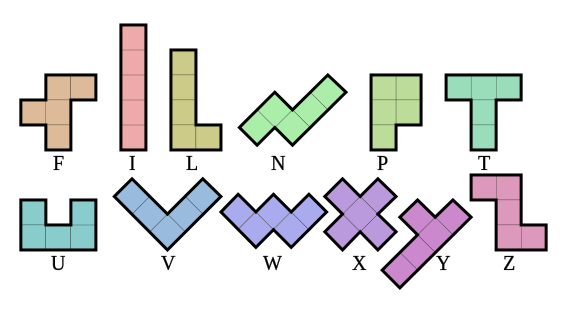
\includegraphics[width=0.45\textwidth]{media/pentomino.png}
    \caption{The twelve pentominoes used in our experiments.}
    \label{fig:pentominoes}
\end{wrapfigure}


\subsection{2D-Tetris Training}

\subsection{Training the Deep Q Network agent}

We adopt a Deep Q Network agent (DQN) with value-based approach in which every legal \texttt{(rotation,,column)} pair is scored by a three-layer multilayer perceptron.  The network processes the four-element state through two hidden layers of 64 rectified linear units before emitting a single action value.  All parameters are initialised with Xavier uniform weights and zero biases.

\paragraph{Experience collection and replay.}
During training the agent interacts with the simulator in an episodic loop in which actions are selected via an epsilon-greedy policy. Epsilon is annealed linearly from one to five times ten to the minus four over three hundred thousand training steps, after which it is held constant.  Every transition tuple is stored in a FIFO replay buffer that holds 30000 entries.  Once the buffer contains at least ten per cent of its capacity, updates commence: a random batch of up to five hundred and twelve samples is drawn, the one-step bootstrap target is computed, and the mean-squared error loss is minimised with Adam at a learning rate of one times ten to the minus four.

\paragraph{Baseline tetromino configuration.}
For the classic seven-piece game we train for three hundred thousand epochs.  All other hyperparameters follow the default values listed above.  Training statistics such as episodic score, pieces placed, cleared lines, and instantaneous loss are logged to TensorBoard each epoch, and human-readable averages are printed every two hundred epochs to monitor stability.

\paragraph{Pentomino extension.}
Introducing the five-block shapes greatly enlarges the action space and amplifies the prevalence of holes and surface roughness.  To compensate we expand the network to a three-layer MLP with 256 hidden units per layer. We also lengthened optimisation to five hundred thousand epochs, allowing the moving epsilon schedule to reach its exploitation regime. Learning rate was tuned to $10^{-4}$, and the batch size was increased to 1024 to accommodate the larger state space. Reward shaping is left intact to keep the comparative analysis between tetromino and pentomino runs straightforward.

\paragraph{Evaluation protocol.}
After training, the checkpoint with the highest validation score is loaded as the agent plays with pure exploitation, selecting the greedy action at every step and recording cumulative score, pieces placed, and cleared lines until game over. The same script can optionally dump an annotated video for qualitative inspection.


\section{Results}
\subsection{Performance in 2D-Tetris Environments}

\paragraph{Learning dynamics with tetrominoes.}
Figure\ref{fig:train4block} plots the evolution of training score over roughly three thousand episodes for the seven-piece game. Around episode two thousand, the curve exhibits a first pronounced jump, after which successive plateaux and spikes appear. The smoothed trace climbs steadily and stabilises near five thousand, while individual trajectories occasionally exceed 1000000 points, highlighting episodic variance once the agent enters the high-score regime.

\paragraph{Learning dynamics with pentominoes.}
In contrast, Figure\ref{fig:train5block} shows that training on the twelve free pentominoes proceeds far more gradually.  The smoothed score starts around ten and only reaches the high thirteens after fifty thousand episodes.  Raw returns are highly volatile throughout, reflecting the highly variable action space and the difficulty of avoiding self-inflicted holes.  Nevertheless the upward trend is monotonic, suggesting that the curriculum and replay settings still permit meaningful gradient signals even in this more demanding domain.

\paragraph{Test performance.}
Agents trained on tetrominoes finish every test game with scores tightly clustered around 15000. They routinely survive until the board approaches the vertical limit and clear multiple four-line combinations per episode.  By contrast, pentomino agents exhibit pronounced instability: median score is roughly 300, with runs ranging from double digits to slightly above seven hundred.  The policy often top-outs early when confronted with asymmetric shapes such as the \emph{F}, \emph{W}, or \emph{X}.

\paragraph{Discussion.}
The stark contrast between the two curves and their associated test scores highlights how sensitive value-based agents remain to the combinatorial growth of the action space.  While the DQN is able to bootstrap from sparse reward and attain human-level play with classic tetrominoes, the same architecture struggles to generalise to pentominoes despite longer training and identical optimisation hyperparameters. 

\begin{wrapfigure}{r}{0.5\textwidth}
    \centering
    \begin{subfigure}{0.45\textwidth}
        \centering
        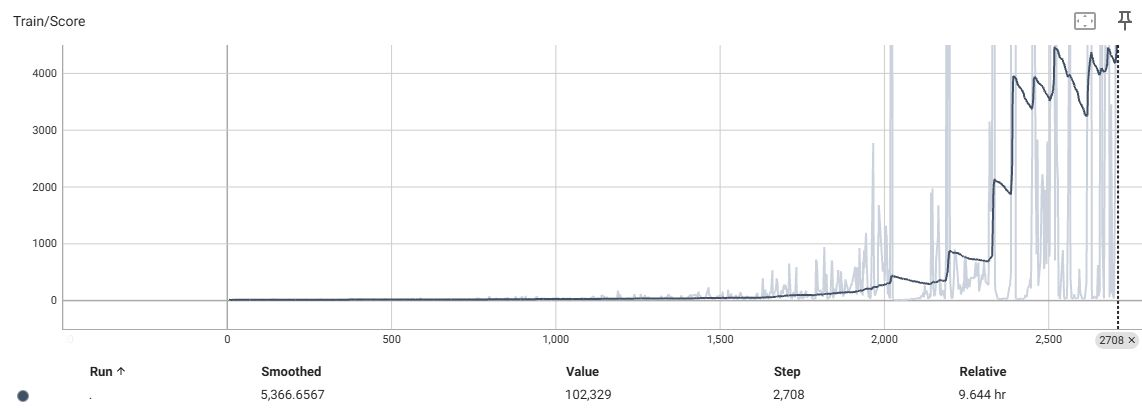
\includegraphics[width=0.90\textwidth]{media/2D_tetramino_training.jpeg}
        \caption{Training curve for 2D-Tetris with Tetraminoes.}
        \label{fig:train4block}
    \end{subfigure}

    \begin{subfigure}{0.45\textwidth}
    \centering
    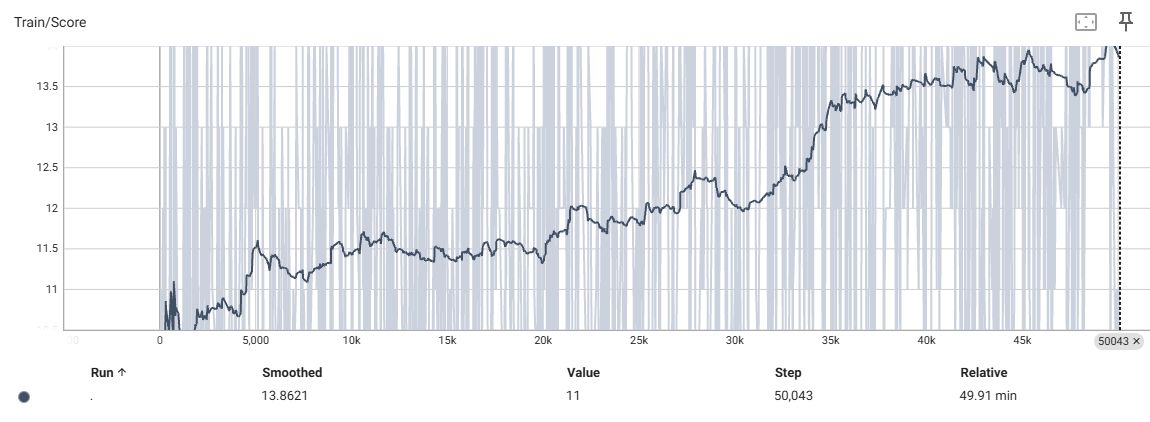
\includegraphics[width=0.90\textwidth]{media/2D_pentamino_training.jpeg}
    \caption{Training curve for 2D-Tetris with Pentominoes.}
    \label{fig:train5block}
    \end{subfigure}

    \caption{The smoothed trace shows the evolution of the average score over the last one hundred episodes, while the raw trace plots the score of each individual episode.}
    \label{fig:2d_training_curves}
\end{wrapfigure}


\input{sections/5-conclusion}

\bibliographystyle{plain}
\bibliography{custom}

\input{sections/appendix}



\end{document}